\immediate\write18{tex celtic.dtx}
\documentclass{ltxdoc}
\usepackage[T1]{fontenc}
\usepackage{trace}
\usepackage{lmodern}
\usepackage{morefloats}
\usepackage{tikz}
\usetikzlibrary{celtic}
\usepackage[numbered]{hypdoc}
\definecolor{lstbgcolor}{rgb}{0.9,0.9,0.9} 
 
\usepackage{listings}
\lstloadlanguages{[LaTeX]TeX}
\lstset{breakatwhitespace=true,breaklines=true,language=TeX}
 
\usepackage{fancyvrb}

\newenvironment{example}
  {\VerbatimEnvironment
   \begin{VerbatimOut}{example.out}}
  {\end{VerbatimOut}
   \begin{center}
   \setlength{\parindent}{0pt}
   \fbox{\begin{minipage}{.9\linewidth}
     \lstset{breakatwhitespace=true,breaklines=true,language=TeX,basicstyle=\small}
     \lstinputlisting[]{example.out}
   \end{minipage}}

   \fbox{\begin{minipage}{.9\linewidth}
     \centering
     \input{example.out}
   \end{minipage}}
\end{center}
}

\providecommand*{\url}{\texttt}

\title{The \textsf{celtic} TikZ Library: Documentation}
\author{Andrew Stacey \\ \url{stacey@math.ntnu.no}}
\date{24th May 2014}

\begin{document}

\maketitle

\begin{center}

\begin{tikzpicture}[
  scale=.5,
  celtic path/.style={
    draw,
    double=gray!40,
    red,
    double distance=1mm,
    line width=4pt
  },
  celtic path 1/.style={
    green!50!black,
  },
]
\CelticDrawPath{
  symmetric crossings={
    1,2,-;
    2,1,|;
    4,3,-;
    3,4,|;
  },
  size={8,8},
}
\end{tikzpicture}
\end{center}

\section{Introduction}

This is a little TikZ library for drawing Celtic style knots.
The particular type of Celtic knot (technically, \emph{link}) is very simple and can be specified by listing the ``walls'' within the region of the knot.
From this information, it is possible to build the entire link and thus to tell TikZ how render it.
That is what this library does.


\begin{example}
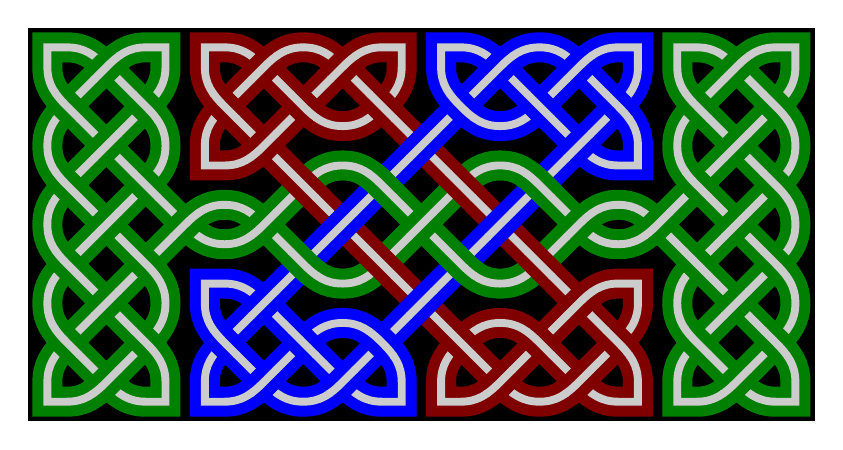
\begin{tikzpicture}[
  scale=.5,
  celtic path/.style={
    draw,
    double=gray!40,
    red,
    double distance=1mm,
    line width=4pt
  },
  celtic path 1/.style={
    green!50!black,
  },
  celtic path 2/.style={
    blue,
  },
  celtic path 3/.style={
    red!50!black,
  },
  celtic surround/.style={
    ultra thick,
    black,
    fill=black
  },
]
\CelticDrawPath{
  symmetric crossings={
    4,1:3,|;
    10,1,|;
    5,4,-;
    8,3,-;
%    10,5,-;
  },
  size={20,10},
  max steps=50
}
\end{tikzpicture}
\end{example}
\end{document}

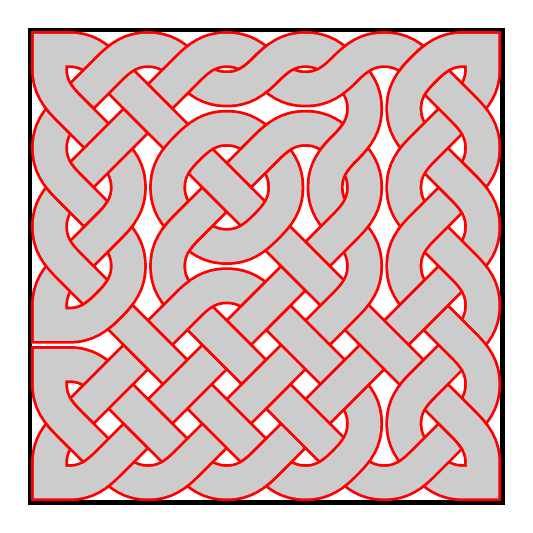
\begin{tikzpicture}[
  scale=.5,
  celtic path/.style={
    draw,
    double=gray!40,
    red,
    double distance=4mm,
    line width=1pt
  },
  celtic path 1/.style={
%    green
  },
  celtic path 2/.style={
%    blue
  },
  celtic surround/.style={
    ultra thick,
    black,
    draw
  },
]
\CelticDrawPath{
  size={12,12},
  crossings={
    5,6,-;
    3,8,|;
    7,8,|;
    5,10,-;
    7,10,-;
    3,6,|;
    9,8,|;
    9,6,|;
    9,10,|;
    1,4,-;
    9,2,|;
  },
  max steps={25}
}
\end{tikzpicture}
\end{document}

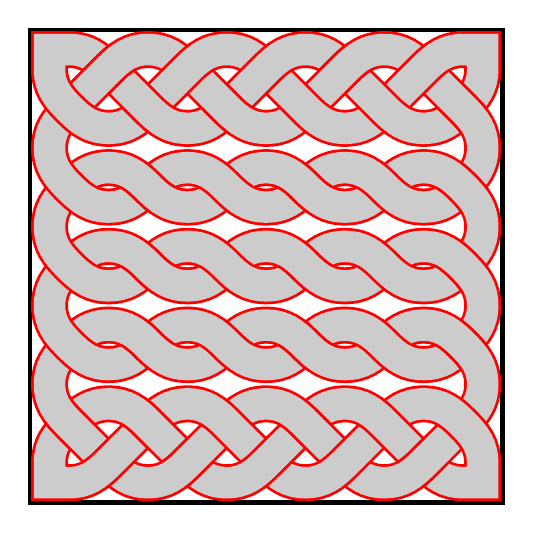
\begin{tikzpicture}[
  scale=.5,
  celtic path/.style={
    draw,
    double=gray!40,
    red,
    double distance=4mm,
    line width=1pt
  },
  celtic surround/.style={
    ultra thick,
    black,
    draw
  },
]
\CelticDrawPath{
  size={12,12},
  symmetric crossings={
    2:10,3:9,-
  },
  at={(1,1)}
}
\end{tikzpicture}

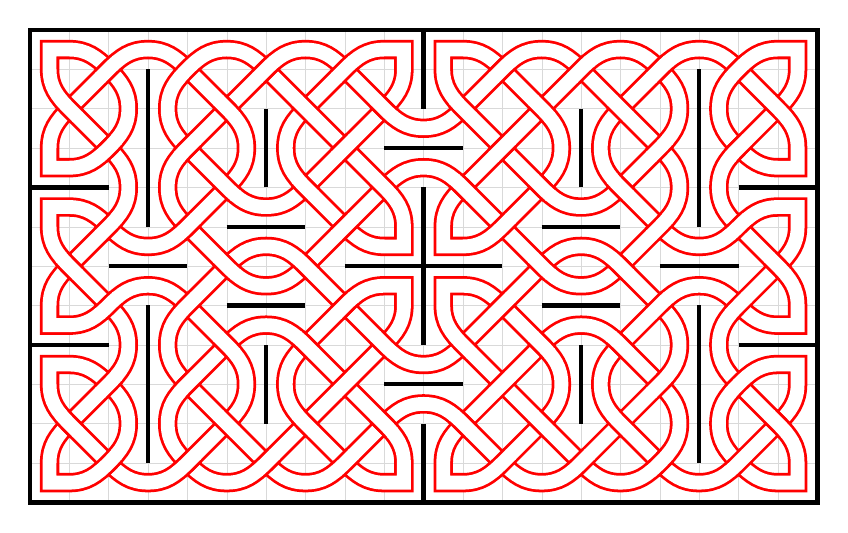
\begin{tikzpicture}[
  scale=.5,
  celtic path/.style={
    draw,
    double=white,
    red,
    double distance=5pt,
    line width=1pt
  },
  celtic bar/.style={
    ultra thick,
    black,
    draw
  },
]
\draw[gray!30,ultra thin] (0,0) grid (20,12);
\CelticDrawPath{
  size={20,12},
  symmetric crossings={
    10,1,|;
    3,2,|;
    3,4,|;
    6,3,|;
    10,5,|;
    10,3,-;
    9,6,-;
    6,5,-;
    3,6,-;
    1,4,-
  },
}
\end{tikzpicture}

\newpage


\begin{tikzpicture}[
  scale=.5,
  celtic path/.style={
    draw,
    double=white,
    red,
    double distance=5pt,
    line width=1pt
  },
  celtic bar/.style={
    ultra thick,
    black,
    draw
  },
]
\CelticDrawPath{
  size={20,38},
  symmetric crossings={
    3,4:34,|;
    4:16,3,-
  },
  ignore symmetric crossings={
    4:10,5:20;
    5:10,4:20
  },
  max steps=1000
}
\end{tikzpicture}



\end{document}

% Local Variables:
% tex-output-type: "pdf18"
% End: